\documentclass[12pt,letterpaper,oneside]{book} 
%\documentclass[12pt,twoside,letterpaper]{book}
% oneside indica que nao � frente e verso

% ---------------------------------------------------------------------------- %
% Pacotes 
\usepackage[T1]{fontenc}
\usepackage[brazil]{babel}
\usepackage[latin1]{inputenc}
\usepackage[pdftex]{graphicx}           % usamos arquivos pdf/png como figuras
\usepackage{setspace}                   % espa�amento flex�vel
\usepackage{indentfirst}                % indenta��o do primeiro par�grafo
\usepackage{makeidx}                    % �ndice remissivo
\usepackage[nottoc]{tocbibind}          % acrescentamos a bibliografia/indice/conteudo no Table of Contents
\usepackage{courier}                    % usa o Adobe Courier no lugar de Computer Modern Typewriter
\usepackage{type1cm}                    % fontes realmente escal�veis
\usepackage{listings}                   % para formatar c�digo-fonte (ex. em Java)
\usepackage{titletoc}
%\usepackage[bf,small,compact]{titlesec} % cabe�alhos dos t�tulos: menores e compactos
\usepackage[fixlanguage]{babelbib}
\usepackage[font=small,format=plain,labelfont=bf,up,textfont=it,up]{caption}
\usepackage[usenames,svgnames,dvipsnames]{xcolor}
\usepackage[a4paper,top=2.54cm,bottom=2.0cm,left=2.0cm,right=2.54cm]{geometry} % margens
%\usepackage[pdftex,plainpages=false,pdfpagelabels,pagebackref,colorlinks=true,citecolor=black,linkcolor=black,urlcolor=black,filecolor=black,bookmarksopen=true]{hyperref} % links em preto
\usepackage[pdftex,plainpages=false,pdfpagelabels,pagebackref,colorlinks=true,citecolor=DarkGreen,linkcolor=NavyBlue,urlcolor=DarkRed,filecolor=green,bookmarksopen=true]{hyperref} % links coloridos
\usepackage[all]{hypcap}                    % soluciona o problema com o hyperref e capitulos
\usepackage[round,sort,nonamebreak]{natbib} % cita��o bibliogr�fica textual(plainnat-ime.bst)
\fontsize{60}{62}\usefont{OT1}{cmr}{m}{n}{\selectfont}

% By David
\usepackage[dvips]{graphicx} 
\usepackage{amsthm}
\usepackage{acronym} 
\usepackage[portugues,ruled,vlined,linesnumbered]{algorithm2e/algorithm2e}
\usepackage{supertabular}

\makeindex  % <== Talvez seja desnecessario

\pagestyle{headings}
\markboth{}{}

% ---------------------------------------------------------------------------- %
% Dimens�es da p�gina (letterpaper)
%\setlength{\paperwidth}{216mm}
%\setlength{\topmargin}{1.3cm}         % deslocamento do topo do texto 
%\setlength\oddsidemargin{0cm}
%\setlength\evensidemargin{0cm}
%\setlength{\parskip}{1.2mm}
%\setlength{\parindent}{4mm}
%\setlength{\textwidth}{135mm}          % largura do texto
%\setlength{\parindent}{0pt}
%\setlength{\textheight}{22cm}
%\setlength{\parskip}{0.2cm}


\newcommand{\eb}{\varepsilon}
\newcommand{\mdp}{\langle\mathcal{S,A},p,r,c\rangle}
\newcommand{\ctlstar}{{\sc ctl}$^\star$}
\newcommand{\ctl}{\sc ctl}
\newcommand{\ltl}{\sc ltl}
\newtheorem{Def}{Defini��o}[chapter]
\newtheorem{Teo}{Teorema}[chapter]
\newtheorem{Ex}{Exemplo}[section]
\newtheorem{Tab}{Tabela}[chapter]

\begin{document}
%\hypersetup{
%pdfauthor = {Suelen Goularte Carvalho},
%pdftitle = {Algo Relacionado a Mobile},
%pdfsubject = {Disserta��o de Mestrado},
%pdfkeywords={Mobile, Computa��o Movel, Celular} % <== Precisa rever o que vai colocar aqui !!!
%pdfcreator = {LaTeX with hyperref package},
%}

\frontmatter

\onehalfspacing
\thispagestyle{empty}
\begin{center}
    \vspace*{0.2cm}
    \textbf{\Large{Primeira parte \\ segunda parte}}\\
	
    \vspace*{1.2cm}
    \Large{Nome do Autor Blah Bleh Blih} \\ 
    
    \vskip 2cm
	\textsc{
	Disserta��o apresentada\\[-0.25cm] 
	ao\\[-0.25cm]
	Instituto de Matem�tica e Estat�stica\\[-0.25cm]
	da\\[-0.25cm]
	Universidade de S�o Paulo\\[-0.25cm]
	para\\[-0.25cm]
	obten��o do t�tulo\\[-0.25cm]
	de\\[-0.25cm]
	Mestre em Ci�ncias}
    
    \vskip 1.5cm
    �rea de Concentra��o: Ci�ncia da Computa��o\\
    Orientadora: Prof$a\over{}$ Dr$a\over$ Nome da orientadora\\

    \vskip 1cm
	\normalsize{}
	
    \vskip 0.5cm
    \normalsize{S�o Paulo, Abril de 2016}

    %\vskip 1cm
        %\Large{\textsc{DRAFT}}
\end{center}

% P�gina de rosto
\newpage
\thispagestyle{empty}
	\begin{center}
    	\vspace*{0.2 cm}
        \textbf{\Large{Primeira parte \\ segunda parte}}\\
	    \vspace*{2 cm}
	\end{center}

	\vskip 2cm

	\begin{flushright}
	Este exemplar corresponde � reda��o\\
	da disserta��o a ser defendida por\\
	Autor Blah Bleh Blih.\\
	\vskip 3cm

	\end{flushright}
	\vskip 4.2cm

	\begin{quote}
	\noindent Banca Examinadora:
	
	\begin{itemize}
		\item {Prof$a\over{}$ Dr$a\over$ Nome da orientadora $-$ IME-USP.}
		\item {Prof. Dr. Nome 222 222 $-$ USP Leste.}
		\item {Prof. Dr. Nome 333 333 $-$ FEI.}
	\end{itemize}
	  
	\end{quote}

\newpage
\thispagestyle{empty}
	\vspace*{12cm}
	\vskip 1cm

	\begin{flushright}
	{\small Dedico esta disserta��o de mestrado aos meus\\
	\ldots \\
	\ldots \\
	\ldots .\\}
	\end{flushright}

	\vspace*{1cm}

	\begin{flushright}
	%{\it ``A Estrada vai sempre em frente''} \\
	%$-$ Bilbo Baggins
	\end{flushright}

\pagebreak


\pagenumbering{roman}

\onehalfspacing
\include{diss-agradecimentos}
%%%%%%%%%%%%%%%%%%%%%%%%%%%%%%%%%%%%%%%%%%%%%%%%%%%%%%%%%%%%%%%%%%%%%%%
\setlength{\parindent}{0pt}
\setlength{\textheight}{22cm}
\setlength{\parskip}{0.2cm}

% Para aumentar o espa�amento entre as linhas
\linespread{1.2}
%%%%%%%%%%%%%%%%%%%%%%%%%%%%%%%%%%%%%%%%%%%%%%%%%%%%%%%%%%%%%%%%%%%%%%%

\chapter*{Resumo}

Lorem ipsum dolor sit amet, consectetur adipiscing elit, sed do eiusmod tempor incididunt ut labore et dolore magna aliqua. Ut enim ad minim veniam, quis nostrud exercitation ullamco laboris nisi ut aliquip ex ea commodo consequat. Duis aute irure dolor in reprehenderit in voluptate velit esse cillum dolore eu fugiat nulla pariatur. Excepteur sint occaecat cupidatat non proident, sunt in culpa qui officia deserunt mollit anim id est laborum. \\

Lorem ipsum dolor sit amet, consectetur adipiscing elit, sed do eiusmod tempor incididunt ut labore et dolore magna aliqua. Ut enim ad minim veniam, quis nostrud exercitation ullamco laboris nisi ut aliquip ex ea commodo consequat. \\

Lorem ipsum dolor sit amet, consectetur adipiscing elit, sed do eiusmod tempor incididunt ut labore et dolore magna aliqua. Ut enim ad minim veniam, quis nostrud exercitation ullamco laboris nisi ut aliquip ex ea commodo consequat. Duis aute irure dolor in reprehenderit in voluptate velit esse cillum dolore eu fugiat nulla pariatur. Excepteur sint occaecat cupidatat non proident, sunt in culpa qui officia deserunt mollit anim id est laborum. \\

Lorem ipsum dolor sit amet, consectetur adipiscing elit, sed do eiusmod tempor incididunt ut labore et dolore magna aliqua. Ut enim ad minim veniam, quis nostrud exercitation ullamco laboris nisi ut aliquip ex ea commodo consequat. Duis aute irure dolor in reprehenderit in voluptate velit esse cillum dolore eu fugiat nulla pariatur. Excepteur sint occaecat cupidatat non proident, sunt in culpa qui officia deserunt mollit anim id est laborum. \\

%\cleardoublepage
\noindent \textbf{Palavras-chave:} planejamento em Intelig�ncia Artificial, reparo de plano, replanejamento.

\chapter*{Abstract}

Lorem ipsum dolor sit amet, consectetur adipiscing elit, sed do eiusmod tempor incididunt ut labore et dolore magna aliqua. Ut enim ad minim veniam, quis nostrud exercitation ullamco laboris nisi ut aliquip ex ea commodo consequat. Duis aute irure dolor in reprehenderit in voluptate velit esse cillum dolore eu fugiat nulla pariatur. Excepteur sint occaecat cupidatat non proident, sunt in culpa qui officia deserunt mollit anim id est laborum. \\

Lorem ipsum dolor sit amet, consectetur adipiscing elit, sed do eiusmod tempor incididunt ut labore et dolore magna aliqua. Ut enim ad minim veniam, quis nostrud exercitation ullamco laboris nisi ut aliquip ex ea commodo consequat. \\

Lorem ipsum dolor sit amet, consectetur adipiscing elit, sed do eiusmod tempor incididunt ut labore et dolore magna aliqua. Ut enim ad minim veniam, quis nostrud exercitation ullamco laboris nisi ut aliquip ex ea commodo consequat. Duis aute irure dolor in reprehenderit in voluptate velit esse cillum dolore eu fugiat nulla pariatur. Excepteur sint occaecat cupidatat non proident, sunt in culpa qui officia deserunt mollit anim id est laborum. \\

Lorem ipsum dolor sit amet, consectetur adipiscing elit, sed do eiusmod tempor incididunt ut labore et dolore magna aliqua. Ut enim ad minim veniam, quis nostrud exercitation ullamco laboris nisi ut aliquip ex ea commodo consequat. Duis aute irure dolor in reprehenderit in voluptate velit esse cillum dolore eu fugiat nulla pariatur. Excepteur sint occaecat cupidatat non proident, sunt in culpa qui officia deserunt mollit anim id est laborum. \\

\noindent \textbf{Keywords:} Artificial Intelligence planning, plan repair, replanning.

\onehalfspacing
\tableofcontents

\chapter{Lista de Abreviaturas}

\begin{acronym}

\acro{ADL}{{\it Action Description Language}} % 
\acro{AIPS}{{\it International Artificial Intelligence Planning Systems}}
\acro{BDD}{{\it Binary Decision Diagram}} %  
\acro{CGP}{{\it Conformant Graphplan}} %
\acro{CSP}{{\it Constraint Satisfaction Problems}}
\acro{CWA}{{\it Closed World Assumption}}
\acro{GPG}{{\it Greedy Planning Graph}} %  
\acro{GPS}{{\it General Problem Solver}}
\acro{HTN}{{\it Hierarchical Task Network}} %  
\acro{IPEM}{{\it Integrated Planning, Exe\-cu\-ti\-on, and Mo\-ni\-to\-ring}} %  
\acro{MDP}{{\it Markov Decision Process}} % 
\acro{PDDL}{{\it Problem Domain Definition Language}} %  
\acro{POCL}{{\it Partial Order Causal Link}}
\acro{POMDP}{{\it Partially Observable Markov Decision Process}} % 
\acro{POP}{{\it Partial Order Planner}} %  
\acro{POPR}{{\it Partial Order Plan Repair}} %  
\acro{PRM}{{\it Probabilistic Roadmap Method}} % 
\acro{SIPE}{{\it System for Iteractive Planning and Exe\-cu\-ti\-on Mo\-ni\-to\-ring}} % 
\acro{STN}{{\it Simple Temporal Netwaorking}}
\acro{STRIPS}{{\it Stanford Research Institute Planning System}} % 
\acro{UCPOP}{{\it Partial Order Planner whose step descriptions include Conditional effects and Universal quantification}}
\acro{VHPOP}{{\it Versatile Heuristic Partial Order Planner}}
%\acro{VHPOP-RE}{VHPOP-RE}


%\acro{ADL}{Linguagem de Descri��o de A��o ({\it Action Description Language})} % 
%\acro{AIPS}{Sistemas de Planejamento em Intelig�ncia Artificial ({\it Artificial Intelligence Planning Systems}) }
%\acro{BDD}{Diagrama de Decis�o Bin�ria ({\it Binary Decision Diagram})} %  
%\acro{CGP}{Grafo de Planejamento Conformante ({\it Conformant Graphplan})} %
%\acro{CPU}{Unidade Central de Processamento ({\it Central Processing Unit})}
%\acro{CSP}{Problemas de Satisfa��o de Restri��es ({\it Constraint Satisfaction Problems})}
%\acro{CWA}{Suposi��o de Mundo Fechado ({\it Closed World Assumption})}
%\acro{GPG}{Grafo de Planejamento Guloso ({\it Greedy Planning Graph})} %  
%\acro{GPS}{Solucionador de Problemas Gen�rico ({\it General Problem Solver})}
%\acro{HTML}{Linguagem de Marca��o de Hipertexto ({\it HyperText Markup Language})}
%\acro{HTN}{Rede Hier�rquica de Tarefas ({\it Hierarchical Task Network})} %  
%\acro{IA}{Intelig�ncia Artificial ({\it Artificial Intelligence})} % 
%% ATEN��O: Na dissertacao nao foi utilizado ``\ac{IA}'' pois nao se desejava que a versao em EN estivesse no texto
%\acro{IPEM}{Planejamento Integrado, Execu��o, e Monitoramento ({\it Integrated Planning, Exe\-cu\-ti\-on, and %Mo\-ni\-to\-ring})} %  
%\acro{MDP}{Processo de Decis�o de Markov ({\it Markov Decision Process})} % 
%\acro{PDDL}{Linguagem de Defini��o de Dom�nio de Planejamento ({\it Problem Domain Definition Language})} %  
%% ATEN��O: Na maior parte disserta��o nao foi utilizado ``\ac{PDDL}'' pois nao se desejava que a versao em PT-BR estivesse no %texto. 
% Somente no Ap�ndice deve aparece a verao por extenso
%\acro{POCL}{V�nculos Causais em Ordem Parcial ({\it Partial Order Causal Link})}
%% ATEN��O: Na disserta��o nao foi utilizado ``\ac{POCL}'' pois se desejava mostrar a sigla em outro formato
%\acro{POMDP}{Processo de Decis�o de Markov Parcialmente Observ�vel ({\it Partially Observable Markov Decision Process})} % 
%\acro{POP}{Planejador de Ordem Parcial ({\it Partial Order Planner})} %  
%\acro{POPR}{Reparo de Plano de Ordem Parcial ({\it Partial Order Plan Repair})} %  
%\acro{PRM}{M�todo Probabil�stico de Roteiro ({\it Probabilistic Roadmap Method})} % 
%\acro{RAM}{Mem�ria de Acesso Aleat�rio ({\it Random Access Memory})}
%\acro{SIPE}{Sistema para Planejamento Iterativo e Monitoramento de Execu��o ({\it System for Iteractive Planning and %Exe\-cu\-ti\-on Mo\-ni\-to\-ring})} % 
%\acro{STN}{Rede Temporal Simples ({\it Simple Temporal Netwaorking})}
%\acro{STRIPS}{Instituto Stanford de Pesquisa em Sistemas de Planejamento ({\it Stanford Research Institute Planning System})} %% 
%% ATEN��O: Na dissertacao nao foi utilizado ``\ac{STRIPS}'' pois nao se desejava que a versao em PT-BR estivesse no texto
%\acro{UCPOP}{Planejador de Ordem Parcial com efeitos Condicionais e quantifica��o Universal ({\it Partial Order Planner whose %step descriptions include Conditional effects and Universal quantification})}
%% ATEN��O: Na disserta��o nao foi utilizado ``\ac{UCPOP}'' pois nao se desejava que a versao em PT-BR estivesse no texto
%\acro{UML}{Linguagem de Modelagem Unificada ({\it Unified Modeling Language})}
%\acro{VHPOP}{Planejador de Ordem Parcial com Versatilidade Heur�stica ({\it Versatile Heuristic Partial Order Planner})}
%%\acro{VHPOP-RE}{VHPOP-RE}

\end{acronym}


\chapter{Lista de S�mbolos}

\begin{supertabular}{ll}


$\Sigma$ & Sistema de transi��o de estados \\


\end{supertabular}


\listoffigures
\listofalgorithms

\mainmatter

%%%%%%%%%%%%%%%%%%%%%%%%%%%%%%%%%%%%%%%%%%%%%%%%%%%%%%%%%%%%%%%%%%%%%%%%%
\onehalfspacing

%%%%%%%%%%%%%%%%%%%%%%%%%%%%%%%%%%%%%%%%%%%%%%%%%%%%%%%%%%%%%%%%%%%%%%%
\setlength{\parindent}{0pt}
\setlength{\textheight}{22cm}
\setlength{\parskip}{0.2cm}

% Para aumentar o espa�amento entre as linhas
\linespread{1.2}
%%%%%%%%%%%%%%%%%%%%%%%%%%%%%%%%%%%%%%%%%%%%%%%%%%%%%%%%%%%%%%%%%%%%%%%

\chapter{Introdu��o}

Smartphones existem desde 1993 por�m nesta �poca o foco era voltado para empresas e suas necessidades. Em 2007 houve o lan�amento do iPhone fabricado pela Apple, o primeiro smartphone voltado ao p�blico em geral. Ao final do mesmo ano o Google revelou seu sistema operacional para dispositivos m�veis, o Android \cite{SmartSociety:13}.

Nos anos que se seguiram diversas grandes empresas como Apple, Google, Blackberry e Microsoft entraram no mercado de smartphones e sistemas operacionais m�veis. Desde ent�o a ado��o do uso de smartphones e mais recentemente outros dispositivos m�veis conhecidos como dispositivos m�veis vest�veis (do ingl�s \textit{wearables}) tais como rel�gios inteligentes, pulseiras, dentre outros, tem crescido espantosamente.

Dentro do mercado de smartphone o Android tem ganhado for�a, o que resulta em mais pessoas usando dispositivos rodando aplica��es android. Desta forma, a demanda por aplicativos tem aumentado de forma acentuada. Logo, a quantidade de aplicativos desenvolvidos tem aumentado em propor��es similares. Isso significa que mais e mais projetos de aplicativos Android vem sendo constru�dos. 

Este crescimento de projetos de aplicativos na plataforma m�vel Android despertou a necessidade e interesse em explorar em mais profundidade quais s�o as particularidades de desenvolvimento nesta plataforma. Este trabalho vem contribuir com uma cole��o de \textit{code smells} validados, particulares a plataforma Android. 

\section{Motiva��o}\index{motiva��o}

A fazer. \\


\section{Objetivos}

A fazer. \\


\section{Abordagem de Solu��o}\index{abordagem}

A fazer. \\


\section{Originalidade e Relev�ncia}\index{originalidade}

A fazer. \\


\section{Organiza��o do Trabalho}\index{organiza��o}

A fazer. \\


 
% -*- root: dissertacao.tex -*-
%%%%%%%%%%%%%%%%%%%%%%%%%%%%%%%%%%%%%%%%%%%%%%%%%%%%%%%%%%%%%%%%%%%%%%%
\setlength{\parindent}{0pt}
\setlength{\textheight}{22cm}
\setlength{\parskip}{0.2cm}

% Para aumentar o espa�amento entre as linhas
\linespread{1.2}
%%%%%%%%%%%%%%%%%%%%%%%%%%%%%%%%%%%%%%%%%%%%%%%%%%%%%%%%%%%%%%%%%%%%%%%

\chapter{Fundamenta��o Te�rica}

Para a compreens�o deste trabalho � importante ter claro a defini��o de 4 itens, s�o eles: \textit{Code Smells}, \textit{Model View Controller}, padr�es e desenvolvimento Android. \\

\section{Aplicativos M�veis}

Aplica��es m�veis s�o \textit{softwares} aplicativos que s�o executados em dispositivos como \textit{smartphones}, \textit{tablets}, \textit{smartwatchs} e mais recentemente outros dispositivos como carros inteligentes e \textit{smart TVs} \cite{MobileSmells:13} \cite{AndroidAuto:16} \cite{AndroidSmart:14}. Este �ltimo apesar de n�o ser um dispositivo m�vel, nos �ltimos anos passou a suportar receber aplica��es que inicialmente foram desenvolvidas para dispositivos m�veis. Aplicativos s�o instalados nos dispositivos atrav�s de lojas de aplicativos onde os usu�rios podem escolher quais aplicativos desejam instalar. \\

Este dispositivos rodam sistemas operacionais feitos especificamente para eles \cite{PercentSmartphoneSales:09-16}. Sistemas operacionais para dispositivos m�veis s�o frequentemente chamados de OS m�vel ou \textit{smartphone} OS ou mesmo plataformas m�veis. Nesta disserta��o usaremos o termo \textbf{Plataforma M�vel} daqui em diante para nos referir a ele. \\

Conforme podemos observar na Figura \ref{fig:mobile-market-share}, at� in�cio de 2010 as plataformas m�veis dominantes eram, da mais dominante para a menos, Symbian, RIM e iOS. No final de 2010 em diante a plataforma m�vel Android ultrapassou sua maior concorrente Symbian em dispositivos vendidos a usu�rios finais e dali em diante at� os dias atuais vem aumentando este n�mero \cite{MobileMarketShares:16}, estando hoje com 84\% da fatia de mercado contra 14\% de sua maior concorrente, o iOS. \\

\begin{figure}[htbp]
	\centering
	\includegraphics[width=0.95\textwidth]{./figuras/mobile-market-share-bars.png}
	\caption{Divis�o global de plataformas m�veis em vendas para usu�rios finais do 1� quadrimestre de 2009 ao 1� quadrimestre de 2016 \cite{PercentSmartphoneSales:09-16}.}
	\label{fig:mobile-market-share}
\end{figure}

Desta forma, as principais plataformas m�veis no momento s�o Android e iOS respectivamente e as proje��es at� 2020 mostram que o Android continuar� na lideran�a \cite{GrowthForecastIDC:16}. 

Existem diversas lojas de aplicativos, dentre elas, existem as oficiais, ou seja, as disponibilizadas pelas fabricantes de cada plataforma. Para Android temos a Google Play Store e para iOS temos a Apple App Store. Na Figura \ref{fig:play-store-apps-09to16} e Figura \ref{fig:apple-store-apps-08to16} podemos observar o aumento da quantidade de aplicativos da Google Play Store e da Apple App Store respectivamente. 

\begin{figure}[ht!]
	\centering
	\includegraphics[width=0.95\textwidth]{./figuras/apple-store-apps-08to16.png}
	\caption[N�mero de aplica��es dispon�veis na Apple App Store de Julho de 2008 a Junho de 2016 \cite{AppInAppleStore:08-16}.]{N�mero de aplica��es dispon�veis na Apple App Store de Julho de 2008 a Junho de 2016 \cite{AppInAppleStore:08-16}.}
	\label{fig:apple-store-apps-08to16}
\end{figure}

\begin{figure}[ht!]
	\centering
	\includegraphics[width=0.95\textwidth]{./figuras/play-store-apps-09to16.png}
	\caption[N�mero de aplica��es dispon�veis na Google Play Store de Dezembro de 2009 a Fevereiro de 2016 \cite{AppInPlayStore:09-16}.]{N�mero de aplica��es dispon�veis na Google Play Store de Dezembro de 2009 a Fevereiro de 2016 \cite{AppInPlayStore:09-16}.}
	\label{fig:play-store-apps-09to16}
\end{figure}

A quantidade de aplicativos dispon�vel nas lojas e a quantidade de instala��es realizadas por usu�rios s�o fortes m�tricas para avaliar o sucesso de uma loja de aplicativos. Segundo o \textit{Wall Street Journal}, no come�o de 2015, a Google Play Store tinha mais de 70\% de downloads de aplicativos que sua principal concorr�nte, a Apple App Store \cite{WSJAppDownloads:15}. � interessante ressaltar que existe uma terceira m�trica de lojas de aplicativos que diz com rela��o a receita gerada, e conforme o mesmo texto do \textit{Wall Street Journal} a Apple App Store gera 70\% mais receita do que a loja da Google.


\section{Maus Cheiros de C�digo}

Mau cheiro de c�digo � uma indica��o superficial que usualmente corresponde a um problema mais profundo em um software. Por si s� um \textit{code smell}, seu termo em ingl�s, n�o � algo ruim, ocorre que frequentemente ele indica um problema mas n�o necess�riamente � o problema em si \cite{CodeSmell:06}. O termo em ingl�s \textit{code smell} foi cunhado pela primeira vez por Kent Beck enquanto ajudava Martin Fowler com o seu livro Refactoring \cite{Refactoring:99} \cite{CodeSmell:06}. \\

\textit{Code Smells} s�o padr�es de c�digo que est�o associados com um design ruim e m�s pr�ticas de programa��o. Diferentemente de erros de c�digo eles n�o resultam em comportamentos erroneos. \textit{Code Smells} apontam para �reas na aplica��o que podem se beneficiar de refatora��es. \cite{MobileSmells:13}. Refatora��o � definido por ``uma t�cnica para reestrutura��o de um c�digo existente, alterando sua estrutura interna sem alterar seu comportamento externo'' \cite{Refactoring:99}. \\

Escolher n�o resolver \textit{code smells} pela refatora��o n�o resultar� na aplica��o falhar mas ir� aumentar a dificuldade de mant�-la. Logo, a refatora��o ajuda a melhorar a manutenabilidade de uma aplica��o \cite{MobileSmells:13}. Uma vez que os custos com manuten��o s�o a maior parte dos custos envolvidos no ciclo de desenvolvimento de software \cite{RefactoringAndImprovements:10}, aumentar a manutenabilidade atrav�s de refatora��o ir� reduzir os custos de um software no longo prazo. 


\section{Model View Controller}

A fazer. \\


\section{Padr�es}

A fazer. \\

\subsection{Formato de Padr�es}

A fazer. \\


\subsection{Formato Alexandrino}

A fazer. \\


\subsection{Formato Adotado}

A fazer. \\

 
%%%%%%%%%%%%%%%%%%%%%%%%%%%%%%%%%%%%%%%%%%%%%%%%%%%%%%%%%%%%%%%%%%%%%%%
\setlength{\parindent}{0pt}
\setlength{\textheight}{22cm}
\setlength{\parskip}{0.2cm}

% Para aumentar o espa�amento entre as linhas
\linespread{1.2}
%%%%%%%%%%%%%%%%%%%%%%%%%%%%%%%%%%%%%%%%%%%%%%%%%%%%%%%%%%%%%%%%%%%%%%%

\chapter{Pesquisa}

Lorem ipsum dolor sit amet, consectetur adipiscing elit. Cras sodales turpis dolor, in porta justo sollicitudin eget. Duis sodales scelerisque viverra. Donec vulputate quam non diam ultricies, nec mattis mauris aliquam. Donec dictum dui ac dictum bibendum. Nunc placerat lobortis euismod. In pellentesque lectus imperdiet eros elementum, et viverra sapien fermentum. Aenean ultricies eu nulla eu molestie. Vivamus in vestibulum eros, rhoncus laoreet magna. Etiam imperdiet vestibulum metus, ac eleifend augue ornare cursus. Pellentesque vitae est purus. Ut eget ex libero. Mauris et sem iaculis, aliquet quam eget, feugiat nisl. Etiam porttitor sollicitudin facilisis. Donec egestas, diam sed tristique vestibulum, leo dolor cursus dui, non placerat lacus erat a augue. Nam ac consequat lectus.

Pellentesque rhoncus lacinia varius. Aliquam consectetur bibendum risus, in egestas tellus. Integer faucibus erat dui, ac interdum risus sodales in. Aenean vel purus mi. Curabitur vulputate dui id velit maximus, a aliquam lacus sodales. Sed condimentum, diam sed fringilla blandit, urna ante cursus quam, quis consectetur quam ipsum in lectus. Donec libero magna, hendrerit sit amet eros id, tempor venenatis nisi. Mauris ac lacus faucibus, dignissim neque id, tincidunt nisi. Pellentesque iaculis leo ut elit pulvinar tristique. Nam enim sapien, posuere vitae gravida gravida, volutpat ac ante. Vestibulum mattis mollis lorem, ut accumsan quam bibendum sed. Pellentesque sodales suscipit lorem, laoreet vehicula velit imperdiet eu. Aenean malesuada tortor eu ligula condimentum consequat. Aliquam at erat diam. Ut in nisi condimentum, faucibus odio ac, dapibus odio. Duis tempor dolor eu mauris euismod, at rhoncus leo luctus. \\

\subsection*{Subsection 1}\index{Lorem!ipsum}

Lorem ipsum dolor sit amet, consectetur adipiscing elit. Cras sodales turpis dolor, in porta justo sollicitudin eget. Duis sodales scelerisque viverra. Donec vulputate quam non diam ultricies, nec mattis mauris aliquam. Donec dictum dui ac dictum bibendum. Nunc placerat lobortis euismod. In pellentesque lectus imperdiet eros elementum, et viverra sapien fermentum. Aenean ultricies eu nulla eu molestie. Vivamus in vestibulum eros, rhoncus laoreet magna. Etiam imperdiet vestibulum metus, ac eleifend augue ornare cursus. Pellentesque vitae est purus. Ut eget ex libero. Mauris et sem iaculis, aliquet quam eget, feugiat nisl. Etiam porttitor sollicitudin facilisis. Donec egestas, diam sed tristique vestibulum, leo dolor cursus dui, non placerat lacus erat a augue. Nam ac consequat lectus.

Pellentesque rhoncus lacinia varius. Aliquam consectetur bibendum risus, in egestas tellus. Integer faucibus erat dui, ac interdum risus sodales in. Aenean vel purus mi. Curabitur vulputate dui id velit maximus, a aliquam lacus sodales. Sed condimentum, diam sed fringilla blandit, urna ante cursus quam, quis consectetur quam ipsum in lectus. Donec libero magna, hendrerit sit amet eros id, tempor venenatis nisi. Mauris ac lacus faucibus, dignissim neque id, tincidunt nisi. Pellentesque iaculis leo ut elit pulvinar tristique. Nam enim sapien, posuere vitae gravida gravida, volutpat ac ante. Vestibulum mattis mollis lorem, ut accumsan quam bibendum sed. Pellentesque sodales suscipit lorem, laoreet vehicula velit imperdiet eu. Aenean malesuada tortor eu ligula condimentum consequat. Aliquam at erat diam. Ut in nisi condimentum, faucibus odio ac, dapibus odio. Duis tempor dolor eu mauris euismod, at rhoncus leo luctus. \\
 

\subsection*{Subsection 2}\index{Lorem!perspiciatis}

Lorem ipsum dolor sit amet, consectetur adipiscing elit. Cras sodales turpis dolor, in porta justo sollicitudin eget. Duis sodales scelerisque viverra. Donec vulputate quam non diam ultricies, nec mattis mauris aliquam. Donec dictum dui ac dictum bibendum. Nunc placerat lobortis euismod. In pellentesque lectus imperdiet eros elementum, et viverra sapien fermentum. Aenean ultricies eu nulla eu molestie. Vivamus in vestibulum eros, rhoncus laoreet magna. Etiam imperdiet vestibulum metus, ac eleifend augue ornare cursus. Pellentesque vitae est purus. Ut eget ex libero. Mauris et sem iaculis, aliquet quam eget, feugiat nisl. Etiam porttitor sollicitudin facilisis. Donec egestas, diam sed tristique vestibulum, leo dolor cursus dui, non placerat lacus erat a augue. Nam ac consequat lectus.

Pellentesque rhoncus lacinia varius. Aliquam consectetur bibendum risus, in egestas tellus. Integer faucibus erat dui, ac interdum risus sodales in. Aenean vel purus mi. Curabitur vulputate dui id velit maximus, a aliquam lacus sodales. Sed condimentum, diam sed fringilla blandit, urna ante cursus quam, quis consectetur quam ipsum in lectus. Donec libero magna, hendrerit sit amet eros id, tempor venenatis nisi. Mauris ac lacus faucibus, dignissim neque id, tincidunt nisi. Pellentesque iaculis leo ut elit pulvinar tristique. Nam enim sapien, posuere vitae gravida gravida, volutpat ac ante. Vestibulum mattis mollis lorem, ut accumsan quam bibendum sed. Pellentesque sodales suscipit lorem, laoreet vehicula velit imperdiet eu. Aenean malesuada tortor eu ligula condimentum consequat. Aliquam at erat diam. Ut in nisi condimentum, faucibus odio ac, dapibus odio. Duis tempor dolor eu mauris euismod, at rhoncus leo luctus. \\


\section{Hip�teses}\index{hipoteses}

Lorem ipsum dolor sit amet, consectetur adipiscing elit. Cras sodales turpis dolor, in porta justo sollicitudin eget. Duis sodales scelerisque viverra. Donec vulputate quam non diam ultricies, nec mattis mauris aliquam. Donec dictum dui ac dictum bibendum. Nunc placerat lobortis euismod. In pellentesque lectus imperdiet eros elementum, et viverra sapien fermentum. Aenean ultricies eu nulla eu molestie. Vivamus in vestibulum eros, rhoncus laoreet magna. Etiam imperdiet vestibulum metus, ac eleifend augue ornare cursus. Pellentesque vitae est purus. Ut eget ex libero. Mauris et sem iaculis, aliquet quam eget, feugiat nisl. Etiam porttitor sollicitudin facilisis. Donec egestas, diam sed tristique vestibulum, leo dolor cursus dui, non placerat lacus erat a augue. Nam ac consequat lectus.

Pellentesque rhoncus lacinia varius. Aliquam consectetur bibendum risus, in egestas tellus. Integer faucibus erat dui, ac interdum risus sodales in. Aenean vel purus mi. Curabitur vulputate dui id velit maximus, a aliquam lacus sodales. Sed condimentum, diam sed fringilla blandit, urna ante cursus quam, quis consectetur quam ipsum in lectus. Donec libero magna, hendrerit sit amet eros id, tempor venenatis nisi. Mauris ac lacus faucibus, dignissim neque id, tincidunt nisi. Pellentesque iaculis leo ut elit pulvinar tristique. Nam enim sapien, posuere vitae gravida gravida, volutpat ac ante. Vestibulum mattis mollis lorem, ut accumsan quam bibendum sed. Pellentesque sodales suscipit lorem, laoreet vehicula velit imperdiet eu. Aenean malesuada tortor eu ligula condimentum consequat. Aliquam at erat diam. Ut in nisi condimentum, faucibus odio ac, dapibus odio. Duis tempor dolor eu mauris euismod, at rhoncus leo luctus. \\


\section{Processo de Pesquisa}

Lorem ipsum dolor sit amet, consectetur adipiscing elit. Cras sodales turpis dolor, in porta justo sollicitudin eget. Duis sodales scelerisque viverra. Donec vulputate quam non diam ultricies, nec mattis mauris aliquam. Donec dictum dui ac dictum bibendum. Nunc placerat lobortis euismod. In pellentesque lectus imperdiet eros elementum, et viverra sapien fermentum. Aenean ultricies eu nulla eu molestie. Vivamus in vestibulum eros, rhoncus laoreet magna. Etiam imperdiet vestibulum metus, ac eleifend augue ornare cursus. Pellentesque vitae est purus. Ut eget ex libero. Mauris et sem iaculis, aliquet quam eget, feugiat nisl. Etiam porttitor sollicitudin facilisis. Donec egestas, diam sed tristique vestibulum, leo dolor cursus dui, non placerat lacus erat a augue. Nam ac consequat lectus.

Pellentesque rhoncus lacinia varius. Aliquam consectetur bibendum risus, in egestas tellus. Integer faucibus erat dui, ac interdum risus sodales in. Aenean vel purus mi. Curabitur vulputate dui id velit maximus, a aliquam lacus sodales. Sed condimentum, diam sed fringilla blandit, urna ante cursus quam, quis consectetur quam ipsum in lectus. Donec libero magna, hendrerit sit amet eros id, tempor venenatis nisi. Mauris ac lacus faucibus, dignissim neque id, tincidunt nisi. Pellentesque iaculis leo ut elit pulvinar tristique. Nam enim sapien, posuere vitae gravida gravida, volutpat ac ante. Vestibulum mattis mollis lorem, ut accumsan quam bibendum sed. Pellentesque sodales suscipit lorem, laoreet vehicula velit imperdiet eu. Aenean malesuada tortor eu ligula condimentum consequat. Aliquam at erat diam. Ut in nisi condimentum, faucibus odio ac, dapibus odio. Duis tempor dolor eu mauris euismod, at rhoncus leo luctus. \\


\subsection{Coleta de Dados}

Lorem ipsum dolor sit amet, consectetur adipiscing elit. Cras sodales turpis dolor, in porta justo sollicitudin eget. Duis sodales scelerisque viverra. Donec vulputate quam non diam ultricies, nec mattis mauris aliquam. Donec dictum dui ac dictum bibendum. Nunc placerat lobortis euismod. In pellentesque lectus imperdiet eros elementum, et viverra sapien fermentum. Aenean ultricies eu nulla eu molestie. Vivamus in vestibulum eros, rhoncus laoreet magna. Etiam imperdiet vestibulum metus, ac eleifend augue ornare cursus. Pellentesque vitae est purus. Ut eget ex libero. Mauris et sem iaculis, aliquet quam eget, feugiat nisl. Etiam porttitor sollicitudin facilisis. Donec egestas, diam sed tristique vestibulum, leo dolor cursus dui, non placerat lacus erat a augue. Nam ac consequat lectus.

Pellentesque rhoncus lacinia varius. Aliquam consectetur bibendum risus, in egestas tellus. Integer faucibus erat dui, ac interdum risus sodales in. Aenean vel purus mi. Curabitur vulputate dui id velit maximus, a aliquam lacus sodales. Sed condimentum, diam sed fringilla blandit, urna ante cursus quam, quis consectetur quam ipsum in lectus. Donec libero magna, hendrerit sit amet eros id, tempor venenatis nisi. Mauris ac lacus faucibus, dignissim neque id, tincidunt nisi. Pellentesque iaculis leo ut elit pulvinar tristique. Nam enim sapien, posuere vitae gravida gravida, volutpat ac ante. Vestibulum mattis mollis lorem, ut accumsan quam bibendum sed. Pellentesque sodales suscipit lorem, laoreet vehicula velit imperdiet eu. Aenean malesuada tortor eu ligula condimentum consequat. Aliquam at erat diam. Ut in nisi condimentum, faucibus odio ac, dapibus odio. Duis tempor dolor eu mauris euismod, at rhoncus leo luctus. \\

\subsection{An�lise dos Dados}

Lorem ipsum dolor sit amet, consectetur adipiscing elit. Cras sodales turpis dolor, in porta justo sollicitudin eget. Duis sodales scelerisque viverra. Donec vulputate quam non diam ultricies, nec mattis mauris aliquam. Donec dictum dui ac dictum bibendum. Nunc placerat lobortis euismod. In pellentesque lectus imperdiet eros elementum, et viverra sapien fermentum. Aenean ultricies eu nulla eu molestie. Vivamus in vestibulum eros, rhoncus laoreet magna. Etiam imperdiet vestibulum metus, ac eleifend augue ornare cursus. Pellentesque vitae est purus. Ut eget ex libero. Mauris et sem iaculis, aliquet quam eget, feugiat nisl. Etiam porttitor sollicitudin facilisis. Donec egestas, diam sed tristique vestibulum, leo dolor cursus dui, non placerat lacus erat a augue. Nam ac consequat lectus.

Pellentesque rhoncus lacinia varius. Aliquam consectetur bibendum risus, in egestas tellus. Integer faucibus erat dui, ac interdum risus sodales in. Aenean vel purus mi. Curabitur vulputate dui id velit maximus, a aliquam lacus sodales. Sed condimentum, diam sed fringilla blandit, urna ante cursus quam, quis consectetur quam ipsum in lectus. Donec libero magna, hendrerit sit amet eros id, tempor venenatis nisi. Mauris ac lacus faucibus, dignissim neque id, tincidunt nisi. Pellentesque iaculis leo ut elit pulvinar tristique. Nam enim sapien, posuere vitae gravida gravida, volutpat ac ante. Vestibulum mattis mollis lorem, ut accumsan quam bibendum sed. Pellentesque sodales suscipit lorem, laoreet vehicula velit imperdiet eu. Aenean malesuada tortor eu ligula condimentum consequat. Aliquam at erat diam. Ut in nisi condimentum, faucibus odio ac, dapibus odio. Duis tempor dolor eu mauris euismod, at rhoncus leo luctus. \\


\section{Escrita dos Code Smells}

Lorem ipsum dolor sit amet, consectetur adipiscing elit. Cras sodales turpis dolor, in porta justo sollicitudin eget. Duis sodales scelerisque viverra. Donec vulputate quam non diam ultricies, nec mattis mauris aliquam. Donec dictum dui ac dictum bibendum. Nunc placerat lobortis euismod. In pellentesque lectus imperdiet eros elementum, et viverra sapien fermentum. Aenean ultricies eu nulla eu molestie. Vivamus in vestibulum eros, rhoncus laoreet magna. Etiam imperdiet vestibulum metus, ac eleifend augue ornare cursus. Pellentesque vitae est purus. Ut eget ex libero. Mauris et sem iaculis, aliquet quam eget, feugiat nisl. Etiam porttitor sollicitudin facilisis. Donec egestas, diam sed tristique vestibulum, leo dolor cursus dui, non placerat lacus erat a augue. Nam ac consequat lectus.

Pellentesque rhoncus lacinia varius. Aliquam consectetur bibendum risus, in egestas tellus. Integer faucibus erat dui, ac interdum risus sodales in. Aenean vel purus mi. Curabitur vulputate dui id velit maximus, a aliquam lacus sodales. Sed condimentum, diam sed fringilla blandit, urna ante cursus quam, quis consectetur quam ipsum in lectus. Donec libero magna, hendrerit sit amet eros id, tempor venenatis nisi. Mauris ac lacus faucibus, dignissim neque id, tincidunt nisi. Pellentesque iaculis leo ut elit pulvinar tristique. Nam enim sapien, posuere vitae gravida gravida, volutpat ac ante. Vestibulum mattis mollis lorem, ut accumsan quam bibendum sed. Pellentesque sodales suscipit lorem, laoreet vehicula velit imperdiet eu. Aenean malesuada tortor eu ligula condimentum consequat. Aliquam at erat diam. Ut in nisi condimentum, faucibus odio ac, dapibus odio. Duis tempor dolor eu mauris euismod, at rhoncus leo luctus. \\


 
% -*- root: dissertacao.tex -*-
%%%%%%%%%%%%%%%%%%%%%%%%%%%%%%%%%%%%%%%%%%%%%%%%%%%%%%%%%%%%%%%%%%%%%%%
\setlength{\parindent}{0pt}
\setlength{\textheight}{22cm}
\setlength{\parskip}{0.2cm}

% Para aumentar o espa�amento entre as linhas
\linespread{1.2}
%%%%%%%%%%%%%%%%%%%%%%%%%%%%%%%%%%%%%%%%%%%%%%%%%%%%%%%%%%%%%%%%%%%%%%%

\chapter{Cat�logo de Code Smells}

A fazer. \\


\section{Especialize sua Tela}

Estou supondo que este possa ser um code smell. A ideia � identificar que uma activity est� com muitas responsabilidades/a��es de usu�rio (vendo a quantidade de listeners em uma mesma activity) e a solu��o seria quebrar em v�rios fragments, de forma a aumentar a coes�o e componentizar para reaproveitar em disposivos de tamanhos de telas diferentes. \\


\section{Code Smell 2}

A fazer. \\


\section{Code Smell 3}

A fazer. \\


\section{Code Smell 4}

A fazer. \\


\section{Code Smell 5}

A fazer. \\ 
%%%%%%%%%%%%%%%%%%%%%%%%%%%%%%%%%%%%%%%%%%%%%%%%%%%%%%%%%%%%%%%%%%%%%%%
\setlength{\parindent}{0pt}
\setlength{\textheight}{22cm}
\setlength{\parskip}{0.2cm}

% Para aumentar o espa�amento entre as linhas
\linespread{1.2}
%%%%%%%%%%%%%%%%%%%%%%%%%%%%%%%%%%%%%%%%%%%%%%%%%%%%%%%%%%%%%%%%%%%%%%%

\chapter{Conclus�o}
\label{cap:conclusao}

Nos �ltimos anos, planejamento automatizado\index{planejamento!automatizado} vem sendo cada vez mais aplicado em problemas pr�ticos de diversas �reas que requerem solu��es confi�veis. Al�m disso, um plano pode falhar durante sua execu��o devido � interfer�ncias de outros agentes (eventos ex�genos). \\

Neste trabalho foram estudadas diferentes abordagens \cite{Kabhampati2005} \cite{Roman2004} \cite{Roman2005} para tratar planejamento n�o\--de\-ter\-mi\-n�s\-ti\-co\index{planejamento!n�o-determin�stico}, por meio de monitora��o de execu��o e reparo de planos. \\

No reparo de planos faz-se a suposi��o de que o custo envolvido no replanejamento completo, a partir do estado que ocorreu a falha � maior do que o reparo do plano tentando-se aproveitar ao m�ximo do plano original. \\


De acordo com \cite{Bernhard1993}, no pior caso, reparar um plano existente n�o � mais eficaz do que um novo replanejamento completo\index{replanejamento}. Entretanto, na pr�tica, o reparo de plano provou ser mais eficaz, uma vez que grande parte do plano ainda � v�lida na maioria dos casos. Como visto no Cap�tulo \ref{cap:implementacao_e_analise_experimental}, utilizar um plano que j� existe, ainda que seja necess�rio ajust�-lo, certamente demanda menos recursos do que construir um plano completamente novo. Al�m disso, em muitos dom�nios pode ser mais dispendioso modificar todo o plano devido a compromissos\index{compromisso} com outros agentes baseados no plano original \cite{Kabhampati2005}. \\

Assim, o objetivo desse trabalho foi investigar as vantagens entre replanejamento e reparo por meio da implementa��o de um sistema de reparo  (VHPOP-RE-H) e compar�-lo com o replanejamento utilizando o planejador cl�ssico VHPOP. \\


\section{Principais contribui��es}

Embora o \ac{VHPOP} \cite{Younes2003} tenha uma implementa��o de dom�nio p�blico, n�o foram
disponibilizados planejadores n�o\--de\-ter\-m�\-nis\-ti\-cos que executem reparo de plano por meio de refinamento reverso ex\-pl�\-ci\-to \cite{Roman2005}. Um dos objetivos do estudo foi prover uma implementa��o das t�cnicas exibidas nas se��es anteriores e possibilitar a compara��o emp�rica com outras abordagens. \\

Outra contribui��o desse trabalho foi o desenvolvimento de uma heur�stica\index{heur�stica} que viabilizasse a implementa��o do modelo de reparo de plano por refinamento reverso. \\

Finalmente, a an�lise experimental mostrou que o sistema VHPOP-RE-H � capaz de reparar, a maioria dos planos, de forma mais eficiente do que os sistemas VHPOP-RE e VHPOP, pois ele gasta menos tempo para encontrar uma solu��o e remove, no m�ximo, o mesmo n�mero de a��es que o replanejamento completo.


\section{Trabalhos futuros}

Algumas extens�es poss�veis desse trabalho s�o:
\begin{itemize}
\item Usar uma heur�stica cl�ssica de busca no espa�o de estados, como por exemplo FF ou HSP, para estimar o custo do replanejamento total.
\item Monitorar se uma ou mais a��es sempre falham em determinadas condi��es, para que o agente deixe de inclu�-las em seus planos.
\item Uma biblioteca de fragmentos de planos\index{fragmentos de planos} \cite{Roman2001}, ou planejamento baseado em casos \cite{Tonidandel2003}.
\item Um conjunto de macro-a��es\index{macro-a��es} \cite{Adi2004} pode melhorar o desempenho em ambientes onde existam informa��es pr�vias, possibilitando, inclusive, a utiliza��o de alguma t�cnica reativa \cite{Castro2005} \cite{Boella2002} para reparo de planos.
\end{itemize}


%\appendix

%%%%%%%%%%%%%%%%%%%%%%%%%%%%%%%%%%%%%%%%%%%%%%%%%%%%%%%%%%%%%%%%%%%%%%%%
\setlength{\parindent}{0pt}
\setlength{\textheight}{22cm}
\setlength{\parskip}{0.2cm}

% Para aumentar o espa�amento entre as linhas
\linespread{1.2}
%%%%%%%%%%%%%%%%%%%%%%%%%%%%%%%%%%%%%%%%%%%%%%%%%%%%%%%%%%%%%%%%%%%%%%%

\chapter{Dom�nios de teste}

\section{PDDL - Linguagem de Defini��o de Do\-m�\-ni\-o de Planejamento}
\label{apendice_pddl}

Em 1998 foi criada a \ac{PDDL}\index{PDDL} \cite{McDermott1998}\cite{McDermott1998a}\cite{McDermott2000}. Esta linguagem tem como principal objetivo representar os dom�nios do mundo real por meio de uma estrutura capaz de ser entendida e interpretada por um planejador. A maioria dos planejadores desenvolvidos hoje s�o capazes de utilizar a \ac{PDDL} como representa��o de entrada do dom�nio para a gera��o de uma solu��o ou de um plano, j� que esta linguagem tornou-se um padr�o na �rea de planejamento autom�tico. A representa��o do modelo do dom�nio deve ser a mais pr�xima poss�vel do dom�nio real, contendo a descri��o das a��es poss�veis, suas pr� e p�s-condi��es, as informa��es sobre o estado inicial do dom�nio e o estado objetivo (metas), para que o planejador possa processar o modelo. \\

Algumas caracter�sticas principais da \ac{PDDL} s�o:


\chapter{Arquitetura do Sistema}
\label{apendice_arquitetura_sistema}

\section{Diagrama de implementa��o}

\begin{center}
  \begin{figure}[ht!]
    \centering
	\label{diagrama_classe}
    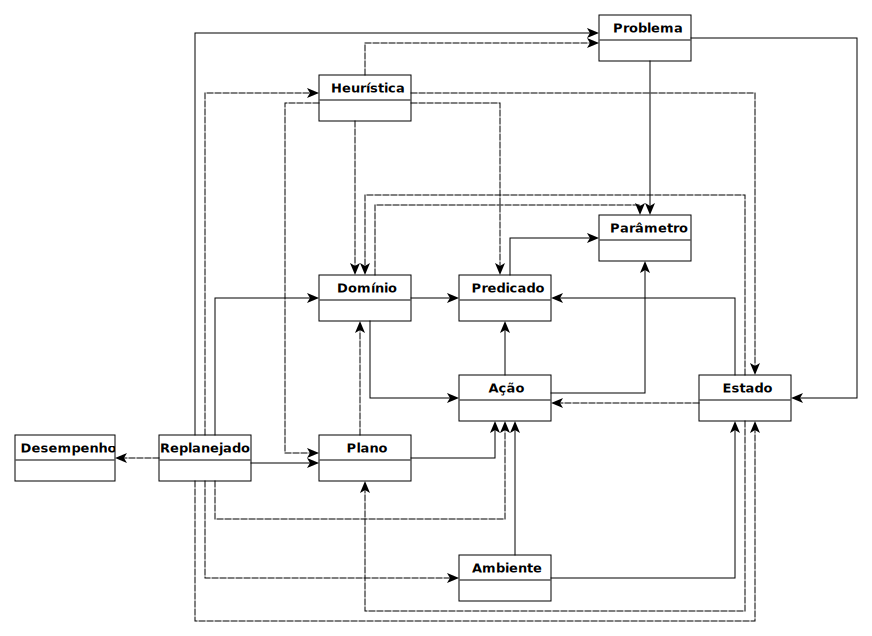
\includegraphics[angle=270,width=1.0\textwidth]{./img/diagrama_classe_sistema.ps}
    \caption[Diagrama de classe do sistema de reparo]{Diagrama de Classe\footnote{Este diagrama segue os conceitos apresentados por \cite{Martin2000}.} do sistema de reparo VHPOP-RE\index{VHPOP-RE}}
  \end{figure}
\end{center}


%%%%%%%%%%%%%%%%%%%%%%%%%%%%%%%%%%%%%%%%%%%%%%%%%%%%%%%%%%%%%%%%%%%%%%%%%

\onehalfspacing
\bibliographystyle{apalike}
\bibliography{diss-bib}

\printindex

\end{document}
